% use lualatex to compile, for some reason xelatex fails for the {Libertinus Serif} font.
\documentclass[11pt]{article}
%\documentclass[11pt]{amsart} % fails on title, date, etc.

% ---------- Fonts (LuaLaTeX / XeLaTeX) ----------
\usepackage{fontspec}
\setmainfont{Libertinus Serif}
%\setmainfont{TeX Gyre Pagella}
%\setsansfont{TeX Gyre Heros}
\setmonofont{Inconsolata}

% ---------- Page layout ----------
\usepackage[a4paper,margin=1.1in]{geometry}

% ---------- Math & theorem setup ----------
\usepackage{amsmath,amssymb,amsthm,mathtools}

\theoremstyle{definition}
\newtheorem{definition}{Definition}

\theoremstyle{plain}
%\newtheorem{theorem}[definition]{Theorem}
\newtheorem{theorem}{Theorem}
\newtheorem{lemma}{Lemma}
\newtheorem{proposition}{Proposition}
\newtheorem{corollary}{Corollary}

\usepackage{xcolor}
\newtheoremstyle{problemstyle} % name
  {3pt} % Space above
  {3pt} % Space below
  {\normalfont} % Body font
  {} % Indent
  {\bfseries\color{blue}} % Theorem head font
  {.} % Punctuation
  { } % Space after head
  {} % Head spec
\theoremstyle{problemstyle}
\newtheorem{problem}{Problem}


\theoremstyle{remark}
\newtheorem*{remark}{Remark}
\renewcommand\qedsymbol{$\blacksquare$}
% the reflection box
\usepackage[framemethod=tikz]{mdframed}
\theoremstyle{definition}
\newtheorem{reflection}{Reflection}
\mdfdefinestyle{reflectionbox}{
  innertopmargin=\topskip,
  roundcorner=5pt,
  linecolor=cyan,
  backgroundcolor=cyan!20,
}
\surroundwithmdframed[style=reflectionbox]{reflection}
% the reflection box
% quotes
\usepackage[autostyle]{csquotes}
\MakeOuterQuote{"}
% quotes

%images
\usepackage{graphicx}
\usepackage{float}
\usetikzlibrary{calc}
%images
% ---------- Typography ----------
\usepackage{microtype}

% ---------- Hyperlinks ----------
\usepackage[hidelinks]{hyperref}

% ---------- Metadata ----------
\title{Notes from \\ \emph{Hyperbolic Functions\\ 
(Topics in Mathematics Translated from the Russian)}
\\ \emph{by V. G. Shervatov}
\\ \emph{(translated by A. Gordon Foster and Coley Mills, Jr.)}}
\author{Kedar Mhaswade}
\date{08 February 2026}

\begin{document}
\maketitle
\begin{reflection}[Introduction]
    These are the author's highly personal notes based on this great book. They may occasionally sound like author's conversation with the reader (or even himself). Even if they are personal and appear in the public domain, they may help the reader, although the author isn't exactly sure how. He wrote them for 0) the love of mathematics and writing 1) \LaTeX{} practice (of writing hopefully readable mathematics, albeit longer than appearing in standard texts), and 2) reliable archival (paper, on which most math is created, tends to get lost) that incurs minimal overhead.

    These notes are interspersed with ``reflection boxes'' like this one. They are meant to express author's `rough' thinking process, of which frustration is often an inseparable part. The author writes mostly in first person for an authentic conversational tone.

    I was lucky to find this book at the time I was discussing the hyperbolic sine and cosine functions with my daughter (who was a high school student then). 
\end{reflection}

\section{The Hyperbolic Rotation}
\subsection{Homothetic Transformations}
\begin{reflection}[The Mathematical Language]
    My computer dictionary flags `homothetic' as a typo, although our understanding of `similarity' in geometry is based on these transformations. Agreed, it is a somewhat esoteric word of a Greek origin. Such transformation means `scaling' in everyday Modern English.  A good definition follows. 
\end{reflection}
\begin{definition}[Homothetic Transformation]\label{def:homothetic-tr}
    If we pick a point $O$ in a plane and a positive real number $k$, and \emph{transform} any other point $A$ to a point $A'$ on the half-line $OA$, such that $\frac{OA'}{OA}=k$ while leaving the point $O$ fixed, then we have carried out a Homothetic Transformation of $A$. See Figure \ref{fig:homothetic-tr}.

    The point $O$ is called the \emph{homothetic center} or \emph{center of similitude}.

    $k$ is called the \emph{homothetic ratio} or \emph{ratio of similitude}.
\end{definition}

\begin{figure}[H]
  \centering
  \includegraphics{images/def-homothetic}
  \caption{Homothetic Transformation of $A$}
  \label{fig:homothetic-tr}
\end{figure}

In arguably simpler terms, we have \emph{scaled} $OA$ by a factor $k$ to $OA'$. Note that $O,A,A'$ are collinear, by definition.

Since $l(OA)=l(OA')\cdot k$, if $k<1$, $l(OA)<l(OA')$ and if $k>1$, $l(OA)>l(OA')$.

\begin{reflection}[Homothetic Transformation of a Straight Line]
    What do we mean by homothetic transformation of a straight line?

    We simply transform every point on that line using the same $O$ and $k$. 

    Do we get a straight line by doing that?

    It appears so, but let's prove that it is so.
\end{reflection}

\begin{problem}\label{prb:straight-line-homothetic-tr}
    Prove that the homothetic transformation of a straight line is a straight line.
\end{problem}
\begin{proof}
    We use step-by-step geometric constructions based on what we are given. First we pick $O$, $k$, and two points $P_1, Q_1$ on a given line $\ell_1$. Let $k>1$. Then, using the definition (\ref{def:homothetic-tr}), we transform $P_1$ to $P_2$, $Q_1$ to $Q_2$.

\begin{figure}[H]
  \centering
    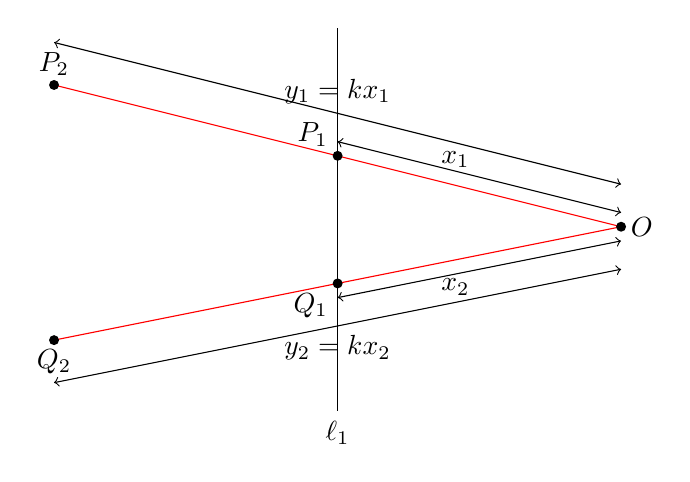
\begin{tikzpicture}[scale=1.2]

    % Origin
    \coordinate (O) at (6,0);

    % Directions
    \coordinate (P2) at (0,1.5);
    \coordinate (Q2) at (0,-1.2);

    % Midpoints (ratio = 0.5)
    \coordinate (P1) at ($(O)!0.5!(P2)$);
    \coordinate (Q1) at ($(O)!0.5!(Q2)$);

    % Rays
        \draw[red] (P2) -- (O);
        \draw[red] (Q2) -- (O);

    % Collinearity
    \draw (Q1) -- (P1);

    % --- Dimension lines (offset) ---

    % Upper ray dimensions
    \draw[<->]
      ($(O)+(0,0.45)$) --
      node[midway, above] {$y_1=kx_1$}
      ($(P2)+(0,0.45)$);

    \draw[<->]
      ($(O)+(0,0.15)$) --
      node[midway, above left] {$x_1$}
      ($(P1)+(0,0.15)$);

    % Lower ray dimensions
    \draw[<->]
      ($(O)+(0,-0.45)$) --
      node[midway, below] {$y_2=kx_2$}
      ($(Q2)+(0,-0.45)$);

    \draw[<->]
      ($(O)+(0,-0.15)$) --
      node[midway, below left] {$x_2$}
      ($(Q1)+(0,-0.15)$);

    % Points
    \fill (O)  circle (1.5pt) node[right] {$O$};
    \fill (P1) circle (1.5pt) node[above left] {$P_1$};
    \fill (P2) circle (1.5pt) node[above] {$P_2$};
    \fill (Q1) circle (1.5pt) node[below left] {$Q_1$};
    \fill (Q2) circle (1.5pt) node[below] {$Q_2$};

    % Line l_1 through P1 and Q1 (extended)
    \draw
    ($(Q1)!2.0!(P1)$) --
    ($(P1)!2.0!(Q1)$)
    node[pos=1.0, below] {$\ell_1$};


  \end{tikzpicture}
    \caption{Construction 1 for Problem [\ref{prb:straight-line-homothetic-tr}]}
    \label{fig:straight-line-homothetic-tr-1}
\end{figure}

We place arbitrarily a point $R_1$ on line $\ell_1$ and transform it using the same $k$ to a point $R_2$. Join $P_2Q_2$ to make $\ell_2$. 

We then ask, ``Is $R_2$ on $\ell_2$ (shown as a dotted line)?''

\begin{figure}[H]
  \centering
    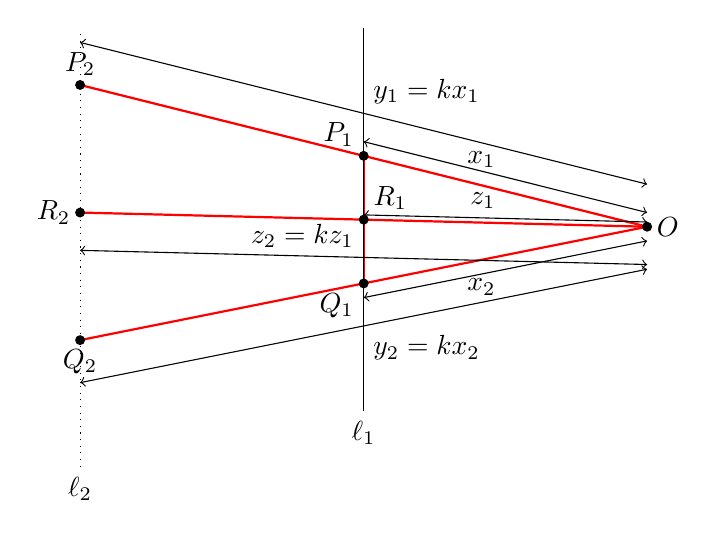
\begin{tikzpicture}[scale=1.2]

    % Origin
    \coordinate (O) at (6,0);

    % Directions
    \coordinate (P2) at (0,1.5);
    \coordinate (Q2) at (0,-1.2);
    \coordinate (R2) at (0,0.15);

    % Midpoints (ratio = 0.5)
    \coordinate (P1) at ($(O)!0.5!(P2)$);
    \coordinate (Q1) at ($(O)!0.5!(Q2)$);
    \coordinate (R1) at ($(P1)!0.5!(Q1)$);

    % Rays
    \draw[red,thick] (P2) -- (O);
    \draw[red,thick] (Q2) -- (O);

    % Collinearity
        \draw[red,thick] (Q1) -- (P1);

    % Join the third pots
        \draw[red,thick] (O) -- (R1);
        \draw[red,thick] (R1) -- (R2);

    % --- Dimension lines (offset) ---

    % Upper ray dimensions
    \draw[<->]
      ($(O)+(0,0.45)$) --
      node[above right] {$y_1=kx_1$}
      ($(P2)+(0,0.45)$);

    \draw[<->]
      ($(O)+(0,0.15)$) --
      node[midway, above left] {$x_1$}
      ($(P1)+(0,0.15)$);

    % Lower ray dimensions
    \draw[<->]
      ($(O)+(0,-0.45)$) --
      node[below right] {$y_2=kx_2$}
      ($(Q2)+(0,-0.45)$);

    \draw[<->]
      ($(O)+(0,-0.15)$) --
      node[midway, below left] {$x_2$}
      ($(Q1)+(0,-0.15)$);

    % Middle ray dimensions
    \draw[<->]
      ($(O)+(0,-0.40)$) --
      node[midway, above left] {$z_2=kz_1$}
      ($(R2)+(0,-0.40)$);

    \draw[<->]
      ($(O)+(0,0.05)$) --
      node[midway, above left] {$z_1$}
      ($(R1)+(0,0.05)$);

    % Points
    \fill (O)  circle (1.5pt) node[right] {$O$};
    \fill (P1) circle (1.5pt) node[above left] {$P_1$};
    \fill (P2) circle (1.5pt) node[above] {$P_2$};
    \fill (Q1) circle (1.5pt) node[below left] {$Q_1$};
    \fill (Q2) circle (1.5pt) node[below] {$Q_2$};
    \fill (R1) circle (1.5pt) node[above right] {$R_1$};
    \fill (R2) circle (1.5pt) node[left] {$R_2$};

    % Line l through P1 and Q1 (extended)
    \draw
    ($(Q1)!2.0!(P1)$) --
    ($(P1)!2.0!(Q1)$)
    node[pos=1.0, below] {$\ell_1$};

    % Line l_2 through P2 and Q2 (extended)
    \draw[dotted]
    ($(Q2)!1.2!(P2)$) --
    ($(P2)!1.5!(Q2)$)
    node[pos=1.0, below] {$\ell_2$};
  \end{tikzpicture}
    \caption{Construction 2 for Problem [\ref{prb:straight-line-homothetic-tr}]}
    \label{fig:straight-line-homothetic-tr-2}
\end{figure}
\begin{reflection}[On Collinearity]
    I have been intrigued about proving collinearity. How do you \emph{prove} whether or not the given points in a plane are collinear? I have clearly forgotten `Elements.'

    Perhaps the easiest approach is to use `similarity of triangles.'

    Or, should I first show that line $P_2Q_2$ ($\ell_2$) is parallel to the line $P_1Q_1$ ($\ell_1$)?

    Should I resort to the Cartesian plane? Here, the idea of `slope' makes it easier, doesn't it? If two segments formed by any three points have the same slope, the points are collinear. Alternatively, with three points, we can make a triangle and argue that if its area is zero, then they are collinear.

    And suddenly an insight came, was it because I recalled the S-A-S test of similarity?
\end{reflection}

Consider $\triangle OP_1Q_1$ and $\triangle OP_2Q_2$. By construction, 1) $OP_1$ and $OP_2$ are proportional and $OQ_1$ and $OQ_2$ are proportional; the ratio of proportionality is the same, $k$, and 2) The included angle, $\angle P_1OQ_1\cong\angle P_2OQ_2$, because they are the same angle.

Therefore, $\triangle OP_1Q_1\sim\triangle OP_2Q_2$.

Therefore, $\angle OP_1Q_1=\angle OP_2Q_2, \angle OQ_1P_1=\angle OQ_2P_2$.

Therefore, $\ell_1\parallel\ell_2$.

Similarly, $\triangle OP_1R_1\sim\triangle OP_2R_2, \triangle OQ_1R_1\sim\triangle OQ_2R_2$.

Therefore, $\ell_1\parallel P_2R_2\parallel R_2Q_2$. This is possible only if $R_2$ is on $\ell_2$.
\end{proof}



\end{document}




\iffalse
\begin{definition}
A set $E \subset \mathbb{R}$ is \emph{bounded} if there exists $M > 0$ such that
\[
|x| \le M \quad \text{for all } x \in E.
\]
\end{definition}

\begin{lemma}
Every finite subset of\/ $\mathbb{R}$ is bounded.
\end{lemma}

\begin{proof}
Let $E = \{x_1, \dots, x_n\}$. Define
\[
M = \max\{|x_1|, \dots, |x_n|\}.
\]
Then $|x| \le M$ for all $x \in E$.
\end{proof}

\begin{theorem}
Every convergent sequence of real numbers is bounded.
\end{theorem}

\begin{proof}
Suppose $x_n \to L$. Then there exists $N$ such that $|x_n - L| < 1$ for all $n \ge N$.
Hence $|x_n| \le |L| + 1$ for $n \ge N$, and the finitely many remaining terms are bounded.
\end{proof}

\begin{remark}
This is the first nontrivial place where the $\varepsilon$--$N$ definition of convergence
actually does work for you, not against you.
\end{remark}
\fi

